\documentclass[11pt, a4paper, twoside]{Thesis}

\usepackage{subcaption}
\usepackage{amsmath}
\usepackage{tocbibind}
\usepackage{multirow}
\usepackage{setspace}
\usepackage{todonotes}
\usepackage{packages/algorithm2e}
\usepackage{textcomp}

\setlength{\parindent}{0.7cm}

\makeatletter
\DeclareRobustCommand\onedot{\futurelet\@let@token\@onedot}
\def\@onedot{\ifx\@let@token.\else.\null\fi\xspace}

\def\eg{\emph{e.g}\onedot} \def\Eg{\emph{E.g}\onedot}
\def\ie{\emph{i.e}\onedot} \def\Ie{\emph{I.e}\onedot}
\def\cf{\emph{c.f}\onedot} \def\Cf{\emph{C.f}\onedot}
\def\etc{\emph{etc}\onedot} \def\vs{\emph{vs}\onedot}
\def\wrt{w.r.t\onedot} \def\dof{d.o.f\onedot}
\def\etal{\emph{et al}\onedot}
\makeatother

\newcommand{\argmax}{\operatornamewithlimits{argmax}}
\newcommand{\argmin}{\operatornamewithlimits{argmin}}
\newcommand{\abs}[1]{\left\lvert#1\right\rvert}
\newcommand{\norm}[1]{\left\lVert#1\right\rVert}
\newcommand{\listofalgorithmes}{\tocfile{\listalgorithmcfname}{loa}}

\begin{document}
% *************** Front matter ***************
\frontmatter

\title  {Rendering and Streaming of
Bidirectional Texture Functions }

\authors  {\texorpdfstring
            {{Oleksandr Sotnychenko}}
            {Oleksandr Sotnychenko}
            }
\addresses  {\groupname\\\deptname\\\univname}  % Do not change this here, instead these must be set in the "Thesis.cls" file, please look through it instead
%\usdate
\date       {Saarbr\"ucken, \today }
\subject    {}
\keywords   {}

\maketitle

%\newpage
%\mbox{}
%\thispagestyle{empty}
%\newpage

\setstretch{1.3}

\thispagestyle{empty}

\section*{Eidesstattliche Erkl\"{a}rung}
Ich erkl\"{a}re hiermit an Eides Statt, dass ich die vorliegende Arbeit selbstst\"{a}ndig verfasst und keine
anderen als die angegebenen Quellen und Hilfsmittel verwendet habe.

\vspace{0.60cm}
\section*{Statement in Lieu of an Oath}
I hereby confirm that I have written this thesis on my own and that I have not used any other media or
materials than the ones referred to in this thesis.
\vspace{1.5cm}

\section*{Sperrvermerk}


\vspace{0.60cm}
\section*{Blocking Notice}

\vspace{3cm}

\begin{flushright}
\noindent Saarbr\"{u}cken, \today
\hfill
Oleksandr Sotnychenko
\end{flushright}

\clearpage  % Declaration ended, now start a new page
%% ----------------------------------------------------------------

\newpage
\mbox{}
\thispagestyle{empty}
\newpage

% The Abstract Page
\addtotoc{Abstract}  % Add the "Abstract" page entry to the Contents
\abstract{
\addtocontents{toc}{\vspace{1em}}  % Add a gap in the Contents, for aesthetics

Bidirectional Texture Function (BTF) is a 6-dimensional function that depends on spatial position on a texture surface and on light and camera views.
An appearance of realistic materials drastically changes with light and camera variations.
 BTF can model reliable presentation of such materials and capture reflectance properties with a wide range of illumination variations.

In this work we present WebGL-based rendering of BTF in a web-browser. 
An ever-growing number of mobile devices that use web-browser implies that rendering must be possible for hardware with very limited capabilities.
Also, due to enormous size of BTF - compression step is inevitable. 
We employ a principal component analysis to compress the data, which allows for rendering of BTF with interactive frame rates. 
To provide immediate feedback to the user we provide a solution to stream the BTF data and to progressively enhance the rendering quality while the data downloads. 






}
\clearpage
%% ----------------------------------------------------------------
\newpage
\mbox{}
\thispagestyle{empty}
\newpage

\setstretch{1.3}  % Reset the line-spacing to 1.3 for body text (if it has changed)

% The Acknowledgements page, for thanking everyone
\acknowledgements{
\addtocontents{toc}{}  % Add a gap in the Contents, for aesthetics    \vspace{1em}


I am deeply grateful to my adviser Jan Sutter for giving me motivation, for sharing his experience with me and for his continuous support in writing my thesis.
I am thankful to my supervisor Prof. Dr. Philipp Slusallek for inspiring me to write the thesis in the field of Computer Graphics and providing me with valuable pieces of advice.
Special thanks go to Kristian Sons and Felix Klein for giving me a continues support and for providing me with directions.

I would like to express my sincere gratitude to Saarland University for providing excellent studying possibilities. 
I am thankful to the German Research Center for Artificial Intelligence for very pleasant working atmosphere.

 Last but not least, I am especially thankful for my parents and friends, who supported me during my studies.






}
\clearpage  % End of the Acknowledgements
%% ----------------------------------------------------------------
\newpage
\mbox{}
\thispagestyle{empty}
\newpage

\thispagestyle{empty}
\emph{To my family.}
\clearpage

\newpage
\mbox{}
\thispagestyle{empty}
\newpage

\setstretch{1}
\begin{spacing}{0.1}
\pagestyle{fancy}
\tableofcontents
\newpage
\listoffigures
\newpage
%\listoftables
%\newpage
%\listofalgorithmes
\end{spacing}

\clearpage

\setstretch{1.3}
% *************** Main matter ***************
\mainmatter

\chapter{Introduction}
\label{chapter:introduction}

One of the main goals in computer graphics is realistic rendering. 
Even though computer graphics is constantly improving, we are still quite away from reality because material representation in a traditional way lack important realistic properties. 
A 2-D texture in conjunction with a shading model is a conventional way to represent material appearances in rendering.
Real-world materials surfaces on the other hand consist of surface meso-structures, i.e. intermediate in between micro and macro structures.
Meso-structures are responsible for fine-scale shadows, self-occlusions, inter-reflection, subsurface scattering and specularities.
Also, reflectance and the look of real-world materials can drastically change when camera and light directions vary.

One of the possible solution to represent such material attributes is to use sophisticated light functions, for instance a Bidirectional Texture Function (BTF). 
 A BTF is a 6-dimensional function that depends on camera and light directions as well as on spatial texture coordinates. 
The BTF conceptually extends traditional 2-D textures by the dependence on light and camera directions.
This function is usually acquired as a data-set of thousands of images that cover discrete light and camera directions.
Due to the enormous size of that data direct renderings even on modern hardware without any compression is impractical.
Fortunately, many techniques exist to deal with the huge size of BTFs, i.e. compression methods.


In this thesis, we use \emph{WebGL} for real-time rendering of BTF in the Web.
Even though 3-D graphics for the Web becoming more and more popular. BTFs are rarely used realistic rendering, due to their huge size and the overall computational effort needed for rendering,
including decompression of the data and interpolation of camera and light directions.
Such demanding computational effort is time consuming, especially for on mobile-devices.

And the problem which arises when rendering BTFs in a Browser is the transmission of the data.
Before rendering on the client side, the transmission of the data has to be finished.
Even the transfer of a compressed BTF data can take a considerable amount of time. 
The compressed BTF can be tens of megabytes in size.
Because users are eager to see a result, especially on the Web, we use a streaming solution to deliver the data as quickly as possibly, while steadily increasing the resulting image.
 \emph{Web-Sockets} are the state of the art technique for streaming and are supported by most of today's browsers.
With \emph{Web-Sockets}  a  full-duplex communication is available for the server and the client, which is faster than traditional HTTP-based methods. 
This promises fast and reliable solution for real-time performance in \emph{WebGL}-based application.

In this thesis we use a PCA for compression, which allows for a considerably good compression ratio with low decompression error.
Also, it is well suited for real-time rendering and streaming.

We implemented WebGL demo web-application and \emph{Web-Sockets} server for streaming purposes.



\section{Related Work}
\label{section:related_work}

Nowadays, Web technologies are able to support WebGL \cite{webgl}, which is a JavaScript API for rendering 3D content.
WebGL provides  vertex and fragment shaders  for creating highly realistic rendering results.
New standards for 3D graphics in context of HTML domain are evolving, for instance such as XML3D \cite{xml3d}.
XML3D allows for embedding 3D graphics into HTML pages. XML3D is based both on XML and WebGL.
It allows for declaring 3D scenes elements in the context of HTML pages.
Web programmers can apply their existing knowledge (i.e. about DOM, XML, CSS) to include 3D graphics in the HTML content by using XML3D.
Currently XML3D  natively supported by  Firefox and Google Chrome browsers on Linux and Windows.
 
Most of previous work that used BTFs for realistic rendering were primarily intended  for offline applications.
However, their approach is not suitable in the context of the Web, due to the data transfer between the server and a client.
  Schwartz \emph{et. al.} \cite{webglbtfstreaming} presented a work in which compressed BTF data is streamed from the server to a client.
 The streaming over the Internet is done by means of HTTP streaming, i.e. the web-application requests the data in small chunks.
 With each new chunk of the BTF data the rendering quality of the 3D object is progressively enhanced.
 We on the other hand, use \emph{Web-Sockets} to improve application performance compared to HTPP streaming, by reducing the network latency and streaming the data in a binary form.

 
Existing BTF compression methods are reviewed by Haindl \emph{et. al.} \cite{haindl, haindl_visual}.
A trade-off has to be made between the rendering quality and compression rate depending on the intended application.
 Our compression method is related to the PCA RF (Principal Component Analysis Reflectance Field) method, which was introduced by Sattler \emph{et. al.} \cite{star2004}.
This method allows for real-time performance with realistic rendering quality. 
Sattler performs PCA on each of the $n$ camera directions separately. We on the other hand, perform PCA on $k$ neighbour camera directions at once.
In Haindl's review \cite{haindl} PCA based methods achieve better or at least equal reconstruction results than most other methods.
Compression rates of PCA methods are not as high as those of other methods. However, those methods, which produce better compression rates, have worse quality than PCA based methods.



\section{Outline}
\label{section:outline}

\begin{figure}[h]
 \centering
 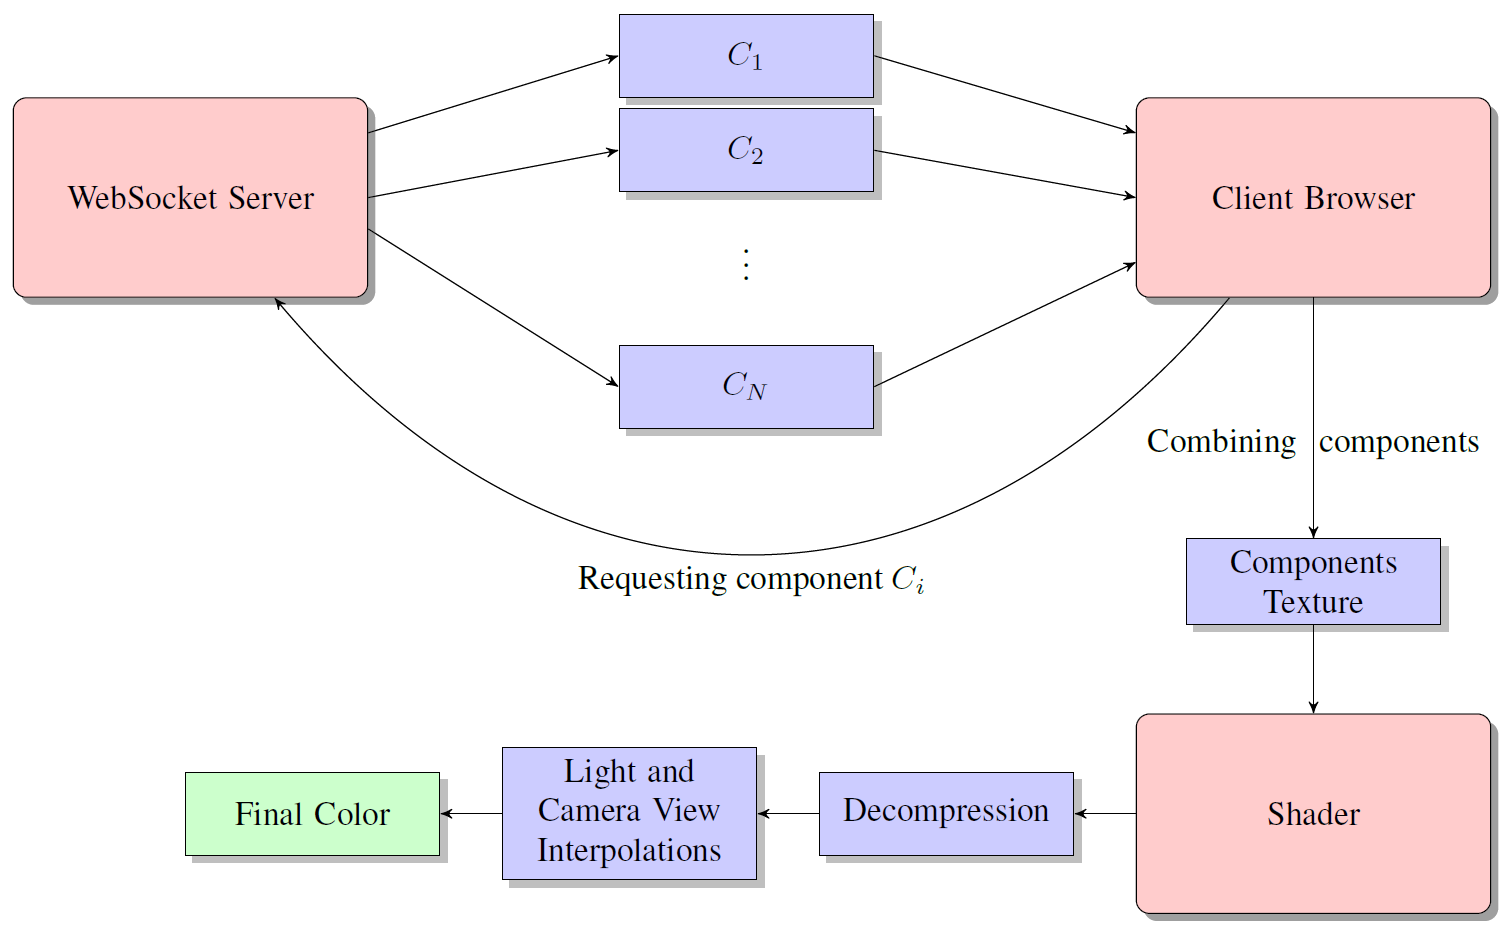
\includegraphics[width=1.0\textwidth]{figures/overview}
 \caption[Model Overview ] {
 	{\bf Model Overview}

	
	}
 \label{fig:overview}
\end{figure}




\clearpage


\chapter{Related Work}
\label{chapter:relatedwork}
\clearpage

\chapter{A hierarchy of scattering functions}
\label{chapter:appearance}

In this chapter we will review a hierarchy of scattering functions. 
Scattering functions describe for a surface how incoming and outgoing directions of the light are related \cite{dong}.
Such functions are possible to measure for a given object.
After obtaining the data, scattering functions can provide all the necessary information to render the material appearance. 
Due to diversity of material properties, different functions were introduced.  
In order to chose suitable scattering function for capturing certain scattering effects for a particular type of material,
it is important to be aware of the hierarchy of scattering functions.

	
\section{Light material interaction}
\label{section:light}	
Before defining any scattering functions of light the basics light-material interaction.
Generally speaking, when light hits a material's surface, a sophisticated light-matter process happens.
Such process depends on physical properties of the material as well as on physical properties of light\cite{wynn}. 
For instance, an opaque surface such as wool will reflect light differently than a smooth surface with high specularities such as metal. 

 When light makes a contact with a material, three types of interactions may occur: light \emph{reflection}, light \emph{absorption} and light \emph{transmittance}. 
 Light \emph{reflection} is the change in direction of light at an interface between two different media so that light returns into the medium from which it originated.
 Light \emph{absorption} is a process when a light is being taken up by a material and transformed into internal energy of the material, for instance thermal energy.
 When a material is transparent, light \emph{transmittance} can occur.
 It means, that the light travels through the material and exits on the opposite side of the object. 
  Figure 2 demonstrates these 3 types of interactions.
  
 Because light is a form of energy, conservation of energy says that \cite{wynn}
 \begin{center} 
\emph{incident light at a surface = light reflected + light absorbed + light transmitted}
 \end{center}
 


\section{General Scattering Function}
\label{section:grf}
 
To define the general scattering function(GSF) imagine the light-wave hitting the surface at time $t_{i}$ and position $x_{i}$ and with wavelength $\lambda_{i}$\cite{star2004}.
 With a given local coordinate system at a surface point, the incoming direction of light can be defined as $(\theta_{i} ,\phi_{i})$.
 Light travels inside the material and exits the surface at position $x_{o}$ and time $t_{o}$, with possibly changed wavelength $\lambda_{o}$ in the outgoing direction $(\theta_{o} ,\phi_{o})$.
  
According to the description we get a GSF
 \begin{center} 
$GSF(t_{i},t_{o},x_{i},x_{0,}\theta_{i} ,\phi_{i},\theta_{o},\phi_{o},\lambda_{i},\lambda_{o})$
 \end{center}
in which  spatial positions $x_{i,o}$ are 2-D variables.
This function describes light interaction for each surface point for any incoming light and outgoing direction at certain time.
The function has 12 parameters! Note that we neglected light transmittance, which would even further complicate the function.


\section{Bidirectional Scattering-Surface Reflectance Distribution Function}
\label{section:BSSRDF}
 Since the measurement, modeling and rendering of a 12-D GSF function is currently not practical, additional assumptions have to be made to simplify the function.
 Usually such assumption are made \cite{star2004}:

\begin{itemize}
 \item light interaction takes zero time ($t_{i}$  = $t_{o}$)
 \item wavelength is separated into the three color bands red, green and blue ($\lambda_{r,g,b}$)
 \item interaction does not change wavelength ($\lambda_{i}= \lambda_{0}$)
\end{itemize}

After mentioned assumptions we get a 8-D bidirectional scattering-surface reflectance distribution function (BSSRDF)
 \begin{center}
$BSSRDF(x_{i},x_{o}\theta_{i} ,\phi_{i}\theta_{o} ,\phi_{o})$
 \end{center}


BSSRDF describes various light interactions for heterogeneous both translucent and opaque materials.
That is why BSSRDF can be used for rendering materials such as skin, marble, milk and other objects which do not look realistic without subsurface scattering. 
Subsurface scattering is a process when light penetrates an object at an incident point, travels inside the object and exists at a different point of the object.

\section{Bidirectional Texture Function}
\label{section:btf}
If we simplify further and assume that

\begin{itemize}
 \item light entering a material exits at the same point $x_{i}=x_{o}$, while internal subsurface scattering is still present
\end{itemize}

we will get a 6-D bidirectional texture function (BTF).

Subsurface scattering, self-occlusion, self-shadowing  are still present, now it just comes pre-integrated, i.e. it can be defined through BSSRDF \cite{star2004}:
 \begin{center}
$ BTF(x,\theta_{i} ,\phi_{i},\theta_{o} ,\phi_{o})=\int_{S}BSSRDF(x_{i},x,\theta_{i} ,\phi_{i},\theta_{o} ,\phi_{o}) dx_{i}$
 \end{center}
  The assumption that $x_{i}=x_{o}$ simplifies measuring, modeling and rendering of the scattering function. 
 As we can see the BTF integrates subsurface scattering from neighbouring surface locations. 

\section{Bidirectional Subsurface Scattering Distribution Function}
\label{section:BSSDF}

Another possible reduction of the 8-D BSSRDF is to assume that we deal with a homogeneous surface \cite{dong}, i.e.
\begin{itemize}
 \item subsurface scattering depends only on relative surface positions of incoming and outgoing light $(x_{i}-x_{o})$
\end{itemize}
  Simply saying it means that scattering do not vary over a surface.
 With such assumption we get a 6D function that known as a bidirectional subsurface scattering
distribution function (BSSDF).
 \begin{center}
$BSSDF(x_{i}-x_{o},\theta_{i} ,\phi_{i},\theta_{o} ,\phi_{o})$
 \end{center}
 BSSDF represents homogeneous materials for which subsurface scattering is a significant feature of their overall appearance.
 For instance, BSSDF accounts for objects such as water, milk, human skin, and marble.

\section{Bidirectional Reflectance Distribution Function}
\label{section:brdf}

If we assume the following for a BSSDF that

\begin{itemize}
 \item there is no spatial variation 
 \item no self-shadowing
 \item no self-occlusion
 \item no inter-reflections
 \item no subsurface scattering
 \item energy conservation
 \item reciprocity  $BRDF(\theta_{i} ,\phi_{i},\theta_{o} ,\phi_{o})$=$BRDF(\theta_{o} ,\phi_{o},\theta_{i} ,\phi_{i})$.
\end{itemize}

 we get a 4-D bidirectional reflectance distribution function (BRDF)
 \begin{center}
$BRDF(\theta_{i} ,\phi_{i},\theta_{o} ,\phi_{o})$.
 \end{center}
Nicodemus et al. \cite{Nicodemus} was the one who proposed the BRDF. 
Two principal properties of the BRDF were introduced, i.e. \emph{energy conservation} and \emph{reciprocity}. 
\emph{Energy conservation} law states that the total amount of outgoing light from a surface cannot exceed the
original amount of light that arrives at the surface \cite{wynn}. 
 \emph{Reciprocity} says that if we swap incoming and outgoing directions BRDF stays the same.
If either of these conditions are not satisfied then such BRDF is called \emph{apparent} BRDF (ABRDF) \cite{abrdf}.

It is quite difficult to create a mathematical model for a BRDF that satisfies reciprocity,
energy conservation and the same time produces realistic images. However, most BRDF's models do not satisfy these conditions and still get plausible rendering results.
For instance, Phong model is the most well-known shading model in computer graphics. 
The traditional Phong model satisfy neither energy conservation nor reciprocity, but can still render many materials realistically plausible.
Usually, such materials are of opaque and flat nature, for example plastic materials.
The Phong model is an empirical model and is designed to fit the original function, often based on simple formulas which were derived from observations.


\section{Spatially Varying Bidirectional Reflectance Distribution Function}
\label{section:svbrdf}
If spatial dependence for BRDF takes place, we get a 6-D spatially varying BRDF (SVBRDF)


 \begin{center}
$SVBRDF(x,\theta_{i} ,\phi_{i},\theta_{o} ,\phi_{o})$.
 \end{center}
 Assumptions are the same as for the BRDF, except now spatial dependence is present.
 
A SVBRDF is closely related to a BTF. The SVBRDF and the BTF almost the same scattering function, the difference is in scattering process. 
Changes in scattering at local position $x$ for the BTF are influenced from neighbouring 3D surface geometry, as a result the self-shadowing, masking and inter-reflections are captured by the BTF.
On the other side, the spatial dependence of a SVBRDF describes variations in the optical properties of a surface \cite{haindl_visual}.


 
A SVBRDF represents structures at micro-scale level, which corresponds to near flat opaque materials. On the other side, a BTF capture structure both at macro and micro scales.
 That means that the BTF takes into account influences from local neighbourhood structures. Even though measurement, compression, rendering are more efficient for the SVBRDF, 
 the BTF can produce better visual results. \cite{haindl_visual}

\section{Summary of scattering functions}
\label{section:attrib}
In practice, an advantage of simpler scattering function is a computation efficiency, 
while a disadvantage is a reduction of visual quality. 
But, development of the graphics hardware is always improving and 
as a result this encourages to use sophisticated scattering functions, which provide improvement in realistic material rendering. 
 
However, a complex material representation introduces additional constraints on the data measurement as well as modeling becomes more challenging.
For instance, till now a GRF has not been measured and still stays as a state-of-the-art problem.
In practice, the appropriate scattering function depends on the specific application.
For instance, a scene with various textures can be rendered with different scattering functions. 
Simpler materials that do not have complex scattering features can be rendered with a 2-D textures in conjunction with BRDFs model. 
If the material cannot be presented realistic without subsurface scattering, masking, self-reflections then typically such materials require high quality representations (BTF,SVBRDF).
However, these advanced material representations are very complex.
In practice a tradeoff between visual quality, measurement, data size and rendering cost is inevitable. 
Ideally high visual quality is preferred with low rendering computational cost.



\clearpage

\chapter{BTF acquisition}
\label{chapter:acquisition}

BTF acquisition is not an easy task as it requires time for acquiring and post-processing the data, and also resources are needed to create acquisition setup.
There are only a few measurement systems \cite{star2004,schwartz,dana,Kaleidoscope,Koudelka,statistical_acq} exist, but as the interest in the realistic material rendering using BTF is growing, measurement systems are developing.
In this chapter we will review how in general BTF data acquisition is made, which post-processing steps are made, and pros and cons of existing measurement systems. 
Also, we will take a look at publicly available BTF datasets.

\section{General acquisition methods}
\label{section:General_acquisition}	
All the mentioned BTF acquisition systems share the same idea in the data acquisition, i.e. capturing the appearance of a flat square slice of the material surface under varying light and camera directions.
The material surface is usually sampled over a hemisphere above the material slice as shown in Figure \ref{fig:acquisition_example}.
Depending on the material reflectance properties sampling distribution may vary, e.g. sampling distribution can be dense in regions where specular peaks in light reflection occur. 
Then, if needed uniform distribution can be made in a post-processing step with a help of interpolation \cite{haindl_visual}.

Digital cameras are used as capturing devices of the material appearance. Depending on the setup the number of cameras can vary.
 If there is only one camera \cite{star2004,statistical_acq,dana}, it usually moves around over the hemisphere above the sample with a help of robotic arm or the rail-trail system \cite{star2004}. 
 The advantage of such approach is that it is less expensive and can suit for low-budget applications.
But, the disadvantage is the positioning errors that can arise, which influence the overall measurement error. 
Depending on the application light sources can be fixed or moveable.

There are approaches which do not involve camera and light source movement at all.
Schwartz et al. \cite{schwartz} developed a novel measurement system which uses a dense array of 151 camera, which are uniformly placed on hemispherical structure.
Flashes of the cameras are used as light sources. Such setup provide high angular and spatial resolutions.

Also, Ngan et al. \cite{statistical_acq} made a setup which does not involve camera movement by placing the planar slices of the material in a form of the pyramid.
Thus, such setup captures the material appearance for 13 different camera views at once. Light directions are sampled by hand-moved electronic flash.
The disadvantage of such setup is that it provides sparse angular resolutions, but depending on the application such approach can be plausible.

The material sample is commonly flat and squared slice, which is placed the holder plate. To conduct automatic post-processing borderline markers are placed on the holder.
Those markers provide the important information for further post-processing steps such as image rectification and registration.


\begin{figure}[h]
 \centering
 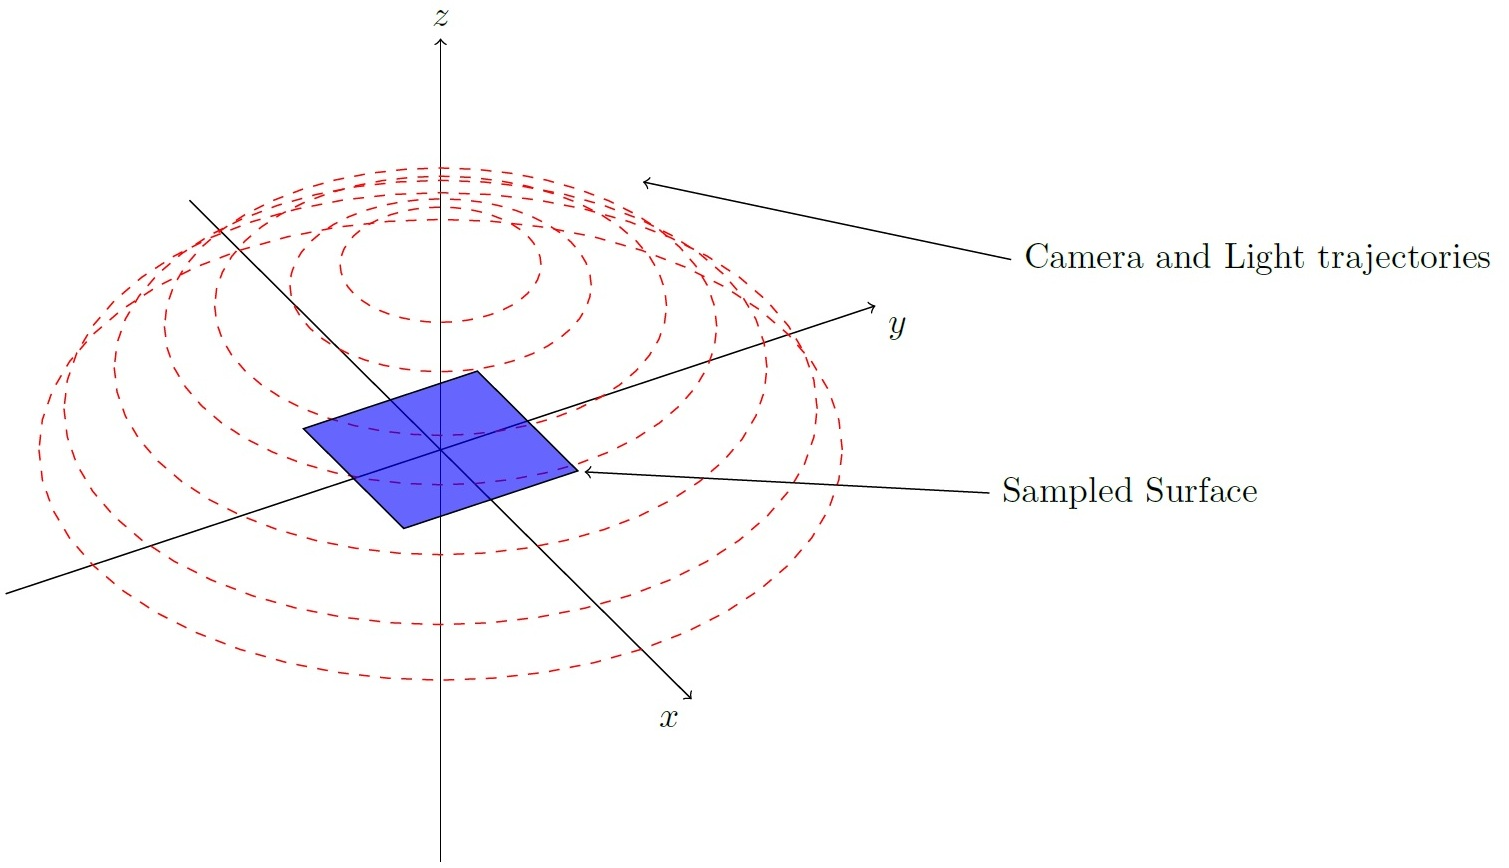
\includegraphics[width=1.0\textwidth]{figures/acquisition}
 \caption[Example of BTF measurement] {
 	{\bf Example of BTF measurement.}

	Camera and light positions share the same trajectories.
	Red dashed circles are the sample positions on the hemisphere. }
 \label{fig:acquisition_example}
\end{figure}

\section{Post-processing steps}
\label{section:Post_processing_acquisition}	
After the measurement is done, the raw data has to be further post-processed, because typically such such data is not ready for further modeling/compression or rendering.
Raw data is a set of images that are not aligned with each other and images are not mutually registered.

When the raw images are obtained under different camera angles $(\theta,\phi)$ they are perspectively distorted \cite{sattler-2003-efficient}.
Thus, sample image have to be aligned with each other and spatially registered to be further exploited.
Firstly, borderline markers that were placed around the material sample on the holder plate aid the automatic detection of the material slice.
Then, after the material slices are detected and cropped, they are ready to for mutual alignment. This process is called  \emph{rectification}. 
\emph{Rectification} is a process which involves projecting all sample images onto the plane which is defined by the frontal view, e.g. $(\theta _{o} =0,\phi _{o}=0)$.
In other words, all normals of sample images have to be aligned with their corresponding camera directions, i.e. as if all sample images were taken from frontal view $(\theta =0,\phi=0)$.
The last step is image \emph{registration}, a process of getting pixel-to-pixel correspondence between the images.
 As, all transformation were done, it is only enough to rescale all images to some equal resolution.


Even after the proper rectification and registering of the measured data, registration errors can be still present between individual camera directions \cite{haindl_visual}. 
 This happens due to structural occlusions of the material surface. Because, of such self-occlusions some geometry structures are not captured by certain camera directions, 
 but can be captured with other camera directions.
 That is why even after rectification images captured from completely different directions are not correctly mutually align. 
Also, registration errors can be caused both by inaccurate camera and material sample positions happened during the measurement processes.
One way to avoid artifacts in rendering caused by registration errors is to employ a compression step separately for each fixed camera positions, i.e. subsets of BTF data. 
 For instance, Sattler et. al. \cite{sattler-2003-efficient} has done this approach.


If needed, further processing steps can be done, for instance \emph{linear edger blending} to reduce tiling artifacts \cite{sattler-2003-efficient}.
Also, typical image processing steps may be employed, e.g. noise reduction filters. 


\section{Publicly available BTF datasets}
\label{section:Publicly_datasets}	

\begin{figure}[h]
 \centering
 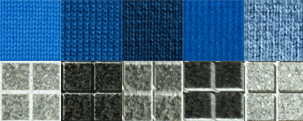
\includegraphics[width=1.0\textwidth]{figures/exampleBTF}
 \caption[Example of BTF measurement] {
 	{\bf BTF example of Bonn Database \cite{btfBonn}.}

	Example how BTF catches rich appearance of the material due to dependencies on light and camera directions. 
	Upper row is a knitted wool, lower is a graved granite stone.}
 \label{fig:exampleBTF}
\end{figure}


The accurate rendering of the material surface is highly depended on the quality of acquired data, especially for BTF.
There are several properties that are vital for reproducing quality rendering results.
The BTF datasets can be distinguished by how well image post-processing were done and how good spatial and angular resolutions are.
So, depending on the application trade-off between high and low spatial or angular resolutions is done.
 For example, some materials with a low range of reflectance may benefit from sparse resolutions, e.g. wool, plastic, etc.
 
 
A pioneer in the BTF acquisition was Dana et. al. \cite{curetDataBase}, who measured 61 materials with fixed light and moving camera aided by a robotic arm. 
Such procedure resulted in a set of images, which can be regarded as a subset of BTF, which is called surface light field (SLF)

{\centering $SLF(x,y,\theta _{i},\phi _{i},\theta _{o},\phi _{o})$ \\}

where $(x,y)$ is a surface point of a flat sampled material, $(\theta _{i},\phi _{i})$ incoming light direction (light direction) and $(\theta _{o},\phi _{o})$ outgoing light direction (camera direction).

Data et. al. \emph{CUReT} database is publicly available \cite{curetDataBase}.
For each measured surface Dana et. al. used 205 different combinations of camera and light directions, which resulted in relatively sparse angular resolution.
 Dana's et. al. BTF database are not rectified, but  the authors provide image coordinates to allow their further rectification. 
 Because, of this limitations such BTF dataset usually used for computer vision purposes, i.e. texture classification  \cite{haindl_visual}.

Based on Dana et. al. BTF measurement system, Sattler from Bonn University made his own measuring system \cite{sattler-2003-efficient}.
 The main difference in that system is that a camera moves on a semi-circle rail around material sample.
Such setup provides spatially rectificated and mutually registered data, with reasonable angular and spatial resolutions. 
Datasets of Bonn University \cite{btfBonn} are publicly available and were used in this thesis.


 Consider Figure \ref{fig:exampleBTF}, which illustrates one of the sampled materials of Bonn database.
The measured surface is being fixed all the time on the sampler holder as shown in Figure \ref{fig:acquisition_example}. For each light position, a camera takes a shot of the material while moving from point to point of the hemisphere.
Bonn database has the same trajectory for camera and light positions, i.e. 81 positions on the hemisphere, which resulted in $81\times81=6561$ total number of acquired images.
After that the sample images were rectificated and registered, resulting in a set of images with spatial resolution $256\times256$.
Typically, the size of one uncompressed BTF is around $1.2$ Gb.







\clearpage

\chapter{BTF Data Representations}
\label{chapter:representations}




Before doing any compression step it is important to chose a suitable data representation for BTF data.
Suitable presentation can enormously influence the final result of BTF rendering.
 Basically, there are two common arrangements for BTF, i.e. as a set of original rectified and registered textures (\emph{image-wise} representation) and a set of ABRDFs (\emph{pixel-wise} representation).
 ABRDF was defined in chapter \ref{section:brdf}. In this case it is called \emph{apparent},
 because BTF includes effects such self-occlusions, sub-surface scattering and other complex effects which violate two basic properties of BRDF.
Both representations can be mathematically expressed as

{\centering $\,\,\,\,\,\,\,BTF_{Texture}=\left \{I_{(\theta_{i} ,\phi_{i},\theta_{o} ,\phi_{o}) }  \mid  (\theta_{i},\phi_{i},\theta_{o} ,\phi_{o})\in M \right \}$\\}
{\centering $\,\,\,\,\,\,\,\,\,\,\,\,\,\,\,\,BTF_{ABRDF}=\left \{P_{(x) } \,\,\,\,\,\,\,\,\,\,\,\,\,\,\,\,\,\,\mid  (x)\in I_{(\theta_{i} ,\phi_{i},\theta_{o} ,\phi_{o})}\subset \mathbb{N}^{2}\right \}$ \\}


where $M$ denotes a set of images $I_{(\theta_{i} ,\phi_{i},\theta_{o} ,\phi_{o})}$ measured for different light and camera directions $(i,o)$ accordingly.
$BTF_{ABRDF}$ denotes a set of $P_{(x)}$ images, where each of them stores light intensity for a fixed spatial position $x$ for all possible light and camera directions, 
i.e. a domain for a $P_{(x)}$ image is $(n_{i}\times n_{o})\subset \mathbb{N}^{2}$, where $n_{i}$ and $n_{o}$ are number of light and camera directions accordingly.
In our case with Bonn datasets the images are given with $256\times256$ resolution for $81\times81$ directions, 
then the size of one single image for both representations are $\left | I \right | = 3\times256\times256$ and $\left | P \right | = 3\times81\times81$, where $3$ stands for RGB channels.

Basically, one representation, i.e. $BTF_{Texture}$ is used for compression methods that do analysis on the whole sample plane, 
while $BTF_{ABRDF}$ representation allows better pixel-to-pixel comparisons, which can give a big advantage for methods that employ pixel-wise compression, e.g. BRDF based models.
Also, such arrangement provides images with lower variance \cite{haindl}, which can allow better compression results in certain scenarios.
But, anyway both representations posses the same information, and any compression method can use either of them.

 
M{\"u}ller et. al. \cite{mueller-2003-compression, haindl} claim that ABRDF representation works slightly better in comparison to image-wise representation. 
The advantage of ABRDF is that a compression ratio can be 10 times better and reconstruction error is slightly smaller than the image-wise representation.
Also, Borshukov et. al. \cite[Ch.\ 15]{gpu_gems} chose ABRDF representation, claiming that it provides better compression ratio.
The reason why ABRDF provides better compression ratio is because it provides better pixel-to-pixel comparison than image-wise. 
Each variable vector of ABRDF arrangement depends only on a surface complexity \cite{mueller-2003-compression}, i.e. 
on a variation of reflection properties at a spatial point of the surface.
On the contrary, image-wise variable depends on the whole measured image plane, thus it is logical that it may provide lower compression rate due to stronger variations.
After all, we have chosen to employ ABRDF data representation based on above reasons, which allowed us to achieve $1:100$ compression ratio. 

\clearpage

\chapter{BTF compression methods}
\label{chapter:compression_methods}



 BTF data consists of thousands of images, which means single BTF requires lots of storage space.
Bonn  Database \cite{btfBonn} consists of 8-bit PNG images with a resolution of $256\times256$ sampled for $81\times81$ different camera and light directions.
 The uncompressed data occupies approx. 1,2 GB of space. And that is only for one BTF material.
 To render the scene with several BTFs and to achieve acceptable frame-rates becomes practically impossible task, especially for low-end hardware.
 Also, as we intent to render BTF in a web-browser, BTF data would have to be transferred from a server to a client, which means the compact representation of BTF is inevitable in such case.
 For our scenario it is important to chose the right compression method, i.e. the one that can allows real-time decompression, high compression rate while preserving good quality, and separability of compressed BTF data.
 Separability is needed for real-time streaming in a web-browser.  
 As the data is transferred in small chunks during the stream and at some point the rendering has to be refreshed, thus it is inevitable to have the ability to decompress full BTF sample having only partial data.

There are different types of methods applied for compressing the BTF. Those methods can be categorized the following way:

\begin{itemize}
  \item \emph{Analytic methods} group, where BTF is represented by analytic BRDF models. 
Analytic BRDF models are the functions which fit separately each texel of BTF. Such functions store few parameters, thus high real-time performance is easily achieved.
However, these group of methods can suffer from decreased quality \cite{haindl}. Also, it is hard to change parameters in order to control the visual quality. Chapter  \ref{section:analytic_methods}.
   \item \emph{Statistic methods}, which belong to methods that reduce dimensionality based on  statistics, for instance based linear basis decompression method such as PCA (Principal component analysis). 
    PCA based methods are frequently used, because its parameters directly correspond to the trade-off between compression ratio and reconstruction quality.
    Also, PCA is frequently a basis point for some more sophisticated methods \cite{webglbtfstreaming}. Chapter \ref{section:stat_methods}.
   \item \emph{Probabilistic models}, which can spatially enlarge BTF to any arbitrary size without visible discontinuities and extremely compress the original BTF.
   However, the resulted quality usually suits for flat surfaces and there are problems of implementing in GPU for real-time rendering. Chapter \ref{section:prob_methods}.
 \end{itemize}



 \section{Analytic methods}
\label{section:analytic_methods}	
 This group of methods take advantage of ABRDF representation of BTF. 
 There is a large number of techniques which allow compactly represent BRDF, which in essence can be also applied for ABRDF.
 Each texel of BTF, i.e. spatial position of surface are represented as ABRDF. Each of these ABRDFs can be modeled and compressed by any BRDF model.
 
One of the possible ways to model ABRDF is to use \emph{Polynomial Texture  Mapping} (PTM) approach.
Malzbender et. al. \cite{PTM} used this approach which allows for high compression rates and generally good quality. 
However, PTM requires to compute specular and diffuse effects separately. 
PTM model assumes that the input surfaces has to be either diffuse or their specular contribution is separated beforehand.
For BTF it can be quite difficult to separate specular highlights \cite{haindl}.

Haindl et. al. \cite{haindl} applied PTM for a fixed camera positions of BTF, i.e. for reflectance fields (RF).
General formula looks the following way (PTM RF):

{\centering$R_{o}(r,i)\approx a_{0}(r)u_{x}^2+a_{1}(r)u_{y}^2+a_{2}(r)u_{x}u_{y}+a_{3}(r)u_{x}+a_{4}(r)u_{y}+a_{5}(r)$\\}

 where $R_{o}$ is approximated RF for fixed camera direction $o$ and $u_{x},u_{y}$ are projections of the normalized light vector into the local coordinate system $r=(x,y)$.
 Set of all possible $R_{o}$ is the number of all camera positions, i.e. $n_{o}$. 
 Coefficients $a_{p}$ are fitted by the use of \emph{singular value decomposition} SVD for each $R_{o}$ and parameters stored as a spatial map referred to as a PTM.
 
 However, Malzbender et. al. \cite{PTM} claims that this method produce considerable errors for high grazing angles. 
 But, nevertheless this method enables fast rendering and generally suited for smooth material surfaces.
 
 Another model which produces slightly better visual quality is the polynomial extension of one-lobe Lafortune model (PLM).
One-lobe Lafortune model (LM) looks the following way \cite{plm}:

{\centering$Y_{o} (r,i) = \rho_{o,r}(C_{o,r,x}u_{x}+C_{o,r,y}u_{y}+C_{o,r,z}u_{z})_{ }^{n_{o,r}}$\\}

where $w_{i}(\theta_{i}, \phi_{i})=[u_{1},u_{2},u_{3}]^{T}$ is a unit vector pointing to light position.
Parameters $\rho,C_{x},C_{y},C_{z},n$ can be computed with a Levenberg-Marquardt non-linear optimisation algorithm \cite{plm}. 
During testing of this model Filip and Haindl \cite{plm} claim that LM produce unsatisfactory results for complex ABRDFs.
 Thus, the polynomial extension of one-lobe Lafortune was introduced (PLM RF):

{\centering$R_{o}(r,i)\approx  \sum_{j=0}^{n} a_{r,o,i,j}Y_{o}(r,i)^j$\\}



PLM RF solves the problem of bad quality for grazing angles and improves the rendering quality compared to PTM RF.
However, statistic based methods produce even better quality compared to above methods but with lower compression rates.



  \section{Statistic methods}
\label{section:stat_methods}


 \section{Probabilistic models}
\label{section:prob_methods}
\clearpage

\chapter{Interpolation of Unmeasured Directions}
\label{chapter:interpolation}


BTF datasets are measured for discrete number of angles, thus we would need to perform interpolation for unknown not measured angels.
We will employ barycentric coordinates interpolation. 
However, it is very computational heavy, so the following approximation algorithm proposed by Hatka and Haindl \cite{btfblender} will be used.

Assume that we have found triangle $P_{1}P_{2}P_{3}$ which bounds our point P, which we want to interpolate. Figure \ref{fig:acquisition_example} demonstrates hemisphere on which triangle $P_{1}P_{2}P_{3}$ lies.
$Y_{P}$ denotes desired pixel color. 
So, generally speaking linearly interpolation of that pixel will be $Y_{P}=w_{1}Y_{P1} + w_{2}Y_{P2} + w_{1}Y_{P2}$, 
where $Y_{P1},Y_{P2},Y_{P3}$ correspond to measured pixel color of positions $P_{1},P_{2},P_{3}$ accordingly. Weights $w_{1},w_{2},w_{3}$ are normalized and sum up to $1$.

Weights defined as volumes $V_{1},V_{2},V_{3}$ which correspond to $PP_{2}P_{3}O$, $PP_{3}P_{1}O$, $PP_{1}P_{2}O$ tetrahedrons, where $O=(0,0,0)$.
All volumes are normalized, which means $V_{i}=\frac{V_{i}}{\sum_{i=1}^{3}V_{i}}$. Volumes calculated as determinates of $4\times 4$ vectors

{\centering $V_{1}=\frac{1}{6}\left | det(PP_{2}P_{3}O) \right |$ \\}
{\centering $V_{2}=\frac{1}{6}\left | det(PP_{3}P_{1}O) \right |$ \\}
{\centering $V_{3}=\frac{1}{6}\left | det(PP_{1}P_{2}O) \right |$ \\}
\clearpage

\chapter{Streaming}
\label{chapter:streaming}



 





In Section \ref{section:algorithm_step} matrices $U$, $\Sigma$ and $V$ store all the data  needed to render the BTF.
Matrices $\Sigma$ and $V$ are small in size and they are sent in the first place. On the contrary, most of the information is stored in the matrix $U$, which stores principal components.
On the client side before streaming, matrix $U$ is initialized with blank values, for example zeros. 
After the Socket connection is established, the client messages the server to send one component at a time. 
 Each component on the WebSockets server is stored as a PNG image, which provides further compression for the BTF.
When a new component fully transferred to the client, it saved to the matrix $U$ and the rendering of the BTF is refreshed.
With each component the quality of the resulting image is progressively enhanced.
Now, with streaming the client is able to see rendered image just in a few seconds.
All matrices on the client are sent to the shader as PNG images.

 The Figure \ref{fig:streaming} illustrates the described streaming process. 
 Components Texture in the Figure \ref{fig:streaming} is the matrix $U$, which saves the transferred principal components.










\clearpage


\chapter{Implementation}

This chapter describes details, problems and limitations of the thesis implementation part.

The implementation of the demo-application is divided into three main parts: compression, streaming and rendering.
The compression is implemented as a standalone Java application, which compresses BTFs from the Bonn University \cite{btfBonn}.
It is possible to adapt any other BTF databases for our demo-application by resampling BTFs \cite{resampling}.
For streaming we use  Node.js \cite{nodejs} platform.
To integrate 3D graphics into HTML page we use XML3D \cite{xml3d}.
The overall model of the demo application is depicted in Figure \ref{fig:overview}.

\begin{figure}[h]
 \centering
 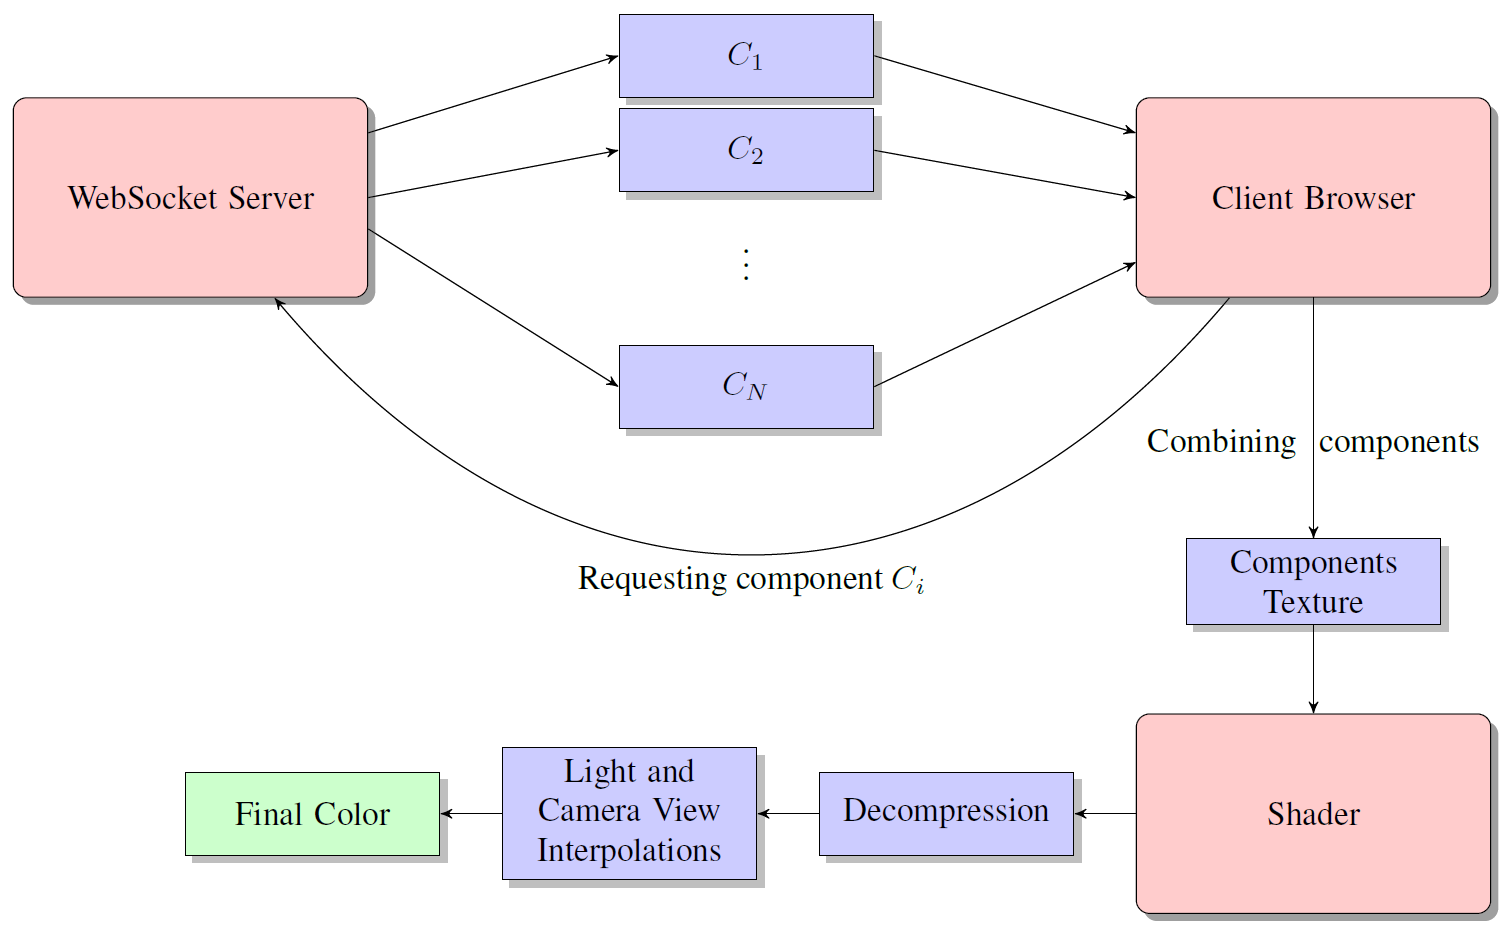
\includegraphics[width=1.0\textwidth]{figures/overview}
 \caption[Model Overview ] {
 	{\bf Model Overview}

	
	}
 \label{fig:overview}
\end{figure}



\section{Compression}
\label{section:impl_compression}

The implementation of the singular value decomposition (SVD) is the main part of the PCA implementation.
 We use \emph{jblas} \cite{jblas} library developed by Mikio Braun. 
 This is a linear algebra library written in Java language, which provides very high performance  \cite{jblas}.
 
The compressed BTFs  have to be sent to the shader. 
  OpenGL Shading Language (GLSL) version 1.0 support uniform arrays, however, they do not fully support dynamic indexing  \cite{glsl}.
Fortunately, it is possible to send arrays of data which are mapped to textures. 
After performing SVD, resulted matrices $U$, $\Sigma$, $V$ are saved as PNG images. (See Chapter \ref{chapter:implementation}).
Values of matrices $U$ and $V$ are in the range of $[-1;1]$.
 Those values have to be mapped to the image domain, i.e. $[0;1]$.
The following function is used to map the values:  

{\centering$f(x)=(x+1)/2$\\}


 Each component of the matrix $U$ is stored as the PNG image.
 For example, if compressed BTF data has $C$ principal components, then this would result in $C$ separate images.
 This is done for streaming purpose, so then principal components can be sent one by one from the server to the client.
 We use  RGBA color space to save four components into the one pixel, because it is possible to do efficient multiplication in the shader by using vector multiplications.
Matrices $V$ and $\Sigma$ are saved in the single shared texture, as they are small in size.

 The matrix $\Sigma$ is a diagonal matrix.
 The values of $\Sigma$ can be bigger than the image color value, i.e. an 8-bit value.
 In practice the values of $\Sigma$ for Bonn University BTFs \cite{btfBonn} are not bigger than four digit number $a_{4}a_{3}a_{2}a_{1}$.
We split the value into two values, i.e. 
 
{\centering$ \underbrace{a_{4}a_{3}}_{R} \underbrace{a_{2}a_{1}}_{G}$\\}
 
It means that two values of $\Sigma$ are mapped into the one pixel, i.e.  one value to RG  channels and the second to BA channels.
If the value of  $\Sigma$ exceed the four digit number, then it is possible to adapt this technique further in the similar manner.


We noticed that in case of Bonn Database \cite{btfBonn} the \emph{jblas} \cite{jblas} library produces relatively sparse values for $U$ and $V$, i.e. close to the zero.
 We scale the data to improve the floating point error caused by mapping of $U$ and $V$ back-and-forth.
The scaling improved the overall decompression error approximately by $5\%$.
 Using the following function we find the scaling factor:
 
 {\centering$ factor(M)=10^{floor(min[log10(min(M)),log10(max(M)]))}$ \\}
 
 where M is the matrix $U$ or $V$. The term $floor(min[log10(min(M)),log10(max(M))])$ calculates the degree with which it is possible to multiply the matrix and preserve the original values range, i.e. $[-1;1]$.
 If it is not possible, the resulting factor will be $1$.
As the decompression is computed as multiplication of $U\Sigma V$, we have to remain the original decompressed BTF values.
We do this by  multiplying each time $\Sigma$ values by the factor $\tfrac{1}{factor(M)}$ if we scale either $U$ or $V$.


 
\section{Streaming}
\label{section:impl_streaming}


We use Node.js \cite{nodejs} as a server side platform, which enables realtime streaming using WebSockets. On top of that, we use BinaryJS \cite{binaryjs} for the binary streaming.
BinaryJS is a framework that uses WebSockets to stream the binary data to the client from the Node.js server.
The server and the client applications are written in JavaScript.



\begin{figure}[h]
 \centering
 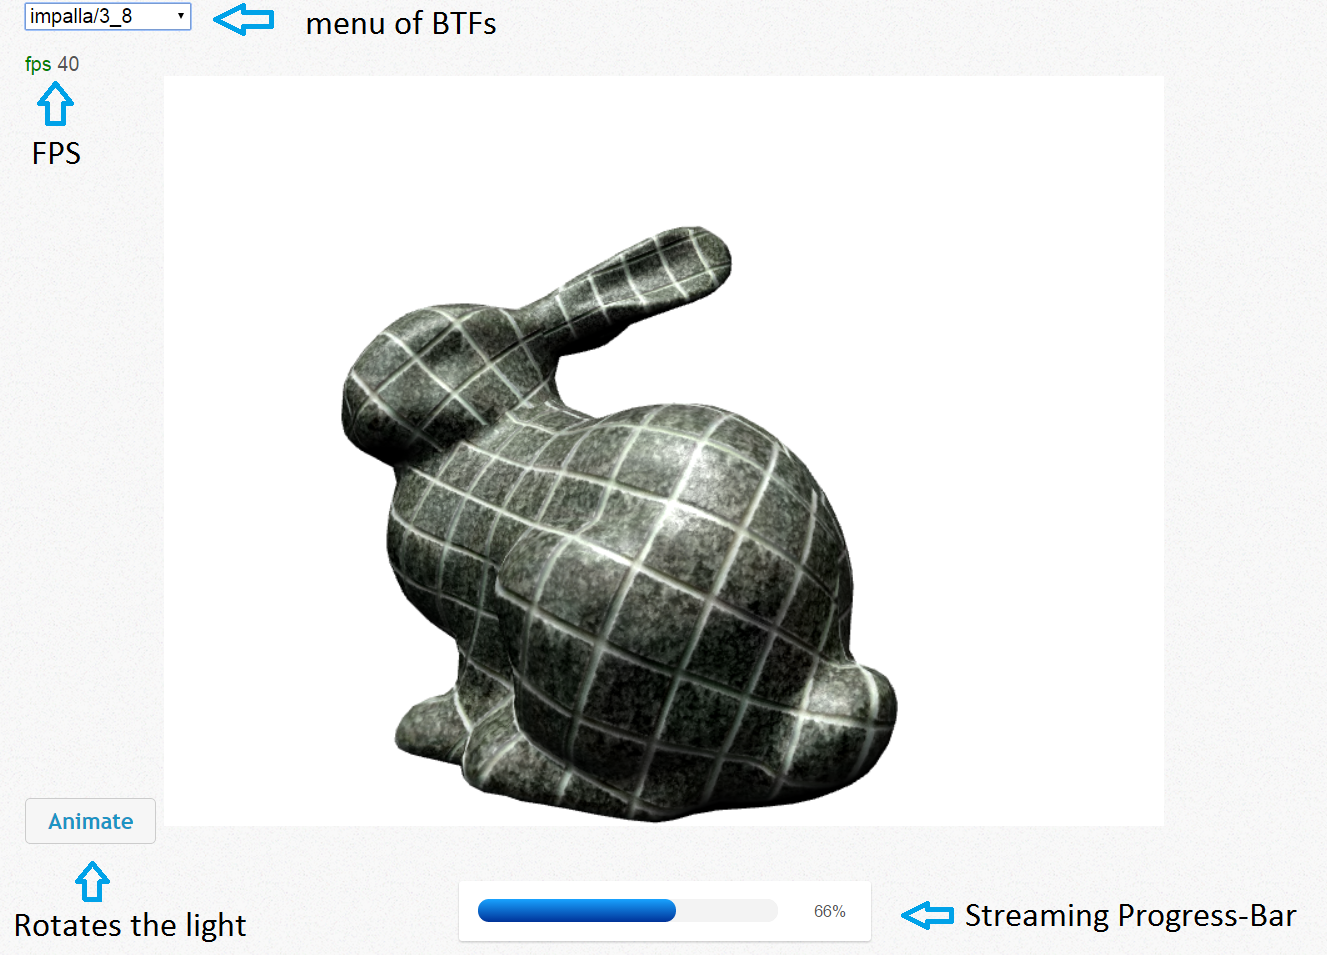
\includegraphics[width=1.0\textwidth]{figures/progress-bar}
 \caption[The streaming progress on the client side] {
 	{\bf The streaming progress on the client side }

 }
 \label{fig:progress-bar}
\end{figure}

We also use Xflow \cite{xflow}, which is a declarative language for data flow processing in realtime.
Xflow is a part of XML3D implementation. We use Xflow for gathering all the transferred principal components and storing them in one common texture $L$. (See Chapter  \ref{section:decompression}).

Consider Figure \ref{fig:streaming} from the Chapter \ref{chapter:streaming} that depicts how the streaming works on practice.
When the user connects to the streaming server and the HTML page loads completely, i.e. all the 3D objects are on the client side, the JavaScript client side sends the message to the Node.js server to start streaming the BTF data.
All the compressed BTFs are located on the Node.js server.
At the start of the stream, we first send texture $R$ and meta data. (See Chapter  \ref{section:decompression}).
Afterwards, each principal component $C_{i}$ are streamed in chunks one by one as PNG images.
Each $C_{i}$ covers all the angular domain, i.e. all the possible camera and light directions.

We decode PNG images using PNG decoder written by Arian Stolwijk \cite{pngreader}. PNG images are decoded to the array of RGB colors and saved to the common texture $L$ in canvas format using Xflow.
Each time the texture $L$ updates the rendering also refreshes.
Even with the first principal component the resulted image looks plausible.
With further components the overall quality of the image improves, i.e. specularities are increasing, small micro-structures become more visible and emphasized.
The user also  able to see the progress-bar of the streaming progress as shown in  Figure \ref{fig:progress-bar}.



Currently the limitation of such streaming approach is the drop of the frame rate when the assembling of the principal components occurs on the client side.
This is caused by the update of the canvas element (texture $L$) each time new component is transmitted to the client.
Also, we did not test the performance of multiple streaming, i.e. if there are several 3D objects that request BTFs at the same time.
 Our current implementation does not support this.
This can be included to the future work. 

\section{Rendering}
\label{section:impl_rendering}


We use XML3D \cite{xml3d} platform to embed 3D graphics into the HTML page. XML3D based on XML and allows for declaring your own 3D scenes and shaders.
XML3D is based on WebGL and JavaScript.

The shader design is depicted in Figure \ref{fig:shader}.
The compressed BTF data comes to the shader in the form of two textures. 
The first texture $L$ stores principal components and the second $R$ stores PCA weights. (See Chapter \ref{section:decompression}).
First, we find three closest directions for the camera and light directions. (See Chapter \ref{chapter:finding_triangle}).
Then, we compute barycentric coordinates for interpolation as described in Chapter \ref{chapter:barycentric}.

\begin{figure}[h]
 \centering
 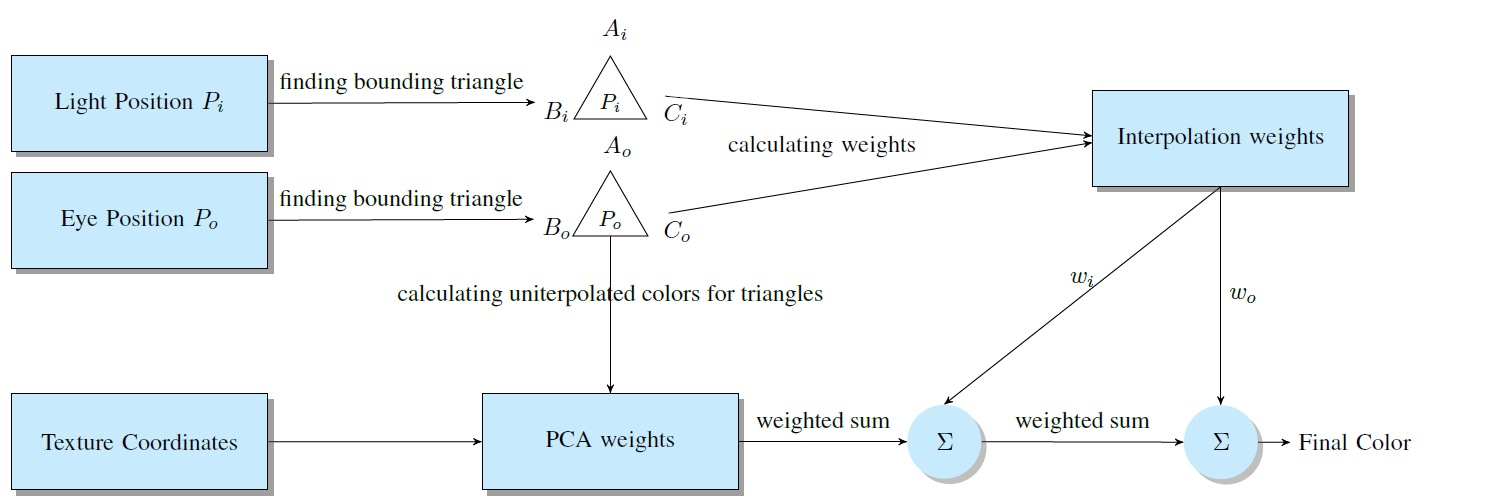
\includegraphics[width=1.0\textwidth]{figures/shader}
 \caption[Shader Design] {
 	{\bf Shader Design }

 }
 \label{fig:shader}
\end{figure}


In the next step we sample the input textures to decompress the needed values for found closest directions.
We have three closest directions per camera and light directions. This means for the interpolation we need to have nine color values. 
For a given texture coordinates $u,v$ we lookup the index of the first principal component, with which it will be possible to start the decompressing.
All the principal components are written linearly in texture $L$, i.e. one by one. 
We have the following mapping to get the needed index:

{\centering$indexL(i,j)= (b*N^2+ (i*N+j))*C$ \\}

where $i=\left \lfloor u*N\right \rfloor$, $j=\left \lfloor v*(N) \right \rfloor$, $b$ is the number of subsets, $N$ is the size of the compressed image and $C$ is number of components.
The parameter $b$ depends on the number of subsets on which PCA is separately done. (See Chapter \ref{section:algorithm_step}).

Texture $R$ stores PCA weights, we lookup the index of suitable compressed image.
The mapping depends on the camera direction $v=(\theta_v,\phi_v)$ and light direction $l=(\theta_l,\phi_l)$.
 It is defined as:

{\centering$ indexR(v,l)=offset(\theta_v,\phi_v)+offset(\theta_l,\phi_l)$\\}

where  $offset(\theta,\phi)=(\tfrac{\theta}{\Delta\theta}+\tfrac{\phi}{\Delta\phi})$, where $\Delta\theta$ and $\Delta\phi$ are quantization step sizes.

When all the indices are computed and textures L and R can be sampled, we decompress the colors as defined in Chapter \ref{section:decompression}.


In a final step we combine nine decompressed colors and early found interpolation weights to get the final color. (See Chapter \ref{chapter:interp_algo}).

The implemented shader has it's own limitations. First of all, the number of principal components has to be fixed for a shader, because GLSL version 1.0 does not allow for dynamic looping \cite{glsl}.
Secondly, the number of principal components are bound by a size of the texture $L$. It means that not all GPUs can handle very big textures. The problem can be fixed by using multiple textures.
But anyway these limitations does not directly influence the performance of the shader, which provides real-time frame rate and performs well even on the mobile devices. (See Figure \ref{fig:progress-bar}).






 




\clearpage

\chapter{Conclusions and Future Work}
\label{chapter:conclusions}
 Bidirectional Texture Functions are currently the best texture representation for the materials 
 that contain high frequencies both in the angular and spatial domain \cite{mueller-2003-compression}.
 Thousands of images has to be taken to sample the appearance of such materials.
 Due to huge sizes of acquired BTFs real-time rendering is impossible to achieve without suitable compression.
 Thus, BTFs still staying in a state of the art in computer graphics. 

\section{Summary}

 In this work we achieved real-time rendering of BTFs in a high quality.
 Considering that we render BTFs in a browser, we managed to reduce the latency that is caused by the data transmission, i.e.
 by streaming  principal components individually.
 We are able to show immediately intermediate rendering results of the textured 3D object.
 We showed experimentally that it is possible to improve the decompression error that was caused by floating point imprecisions.
 The scaling of the compressed BTF data before converting it into the textures improved the decompression error approximately by $5\%$.
 As a result this also improved the real-time frame rates and the compression ratio due to reduction in the number of components used.


Finally, our method is flexible and allows for balancing between the visual quality, memory usage and computational effort.
\section{Future work}
\label{section:future_work}

Based on our results several directions for the future work can be made.
First of all, multiple streaming of BTFs can be implemented.
Secondly, several optimizations of the BTF shader performance can be made.
For instance, it is possible to reduce some of the calculations such as computation of the interpolation weights. 
They can be precomputed and stored in a cube-map \cite{haindl}.
Other calculations such as computation of the bidirectional normals can be precomputed and stored along with a 3D mesh.

Last but not least, there is a room for further compression.
 For instance, it can be achieved by compressing the PCA parameters with wavelet compression \cite{webglbtfstreaming} or with entropy encoding \cite{gpu_gems}. 
However, the decompression cost will grow, but it can be worth if further memory savings are necessary. 
\clearpage


% *************** Bibliography ***************
\bibliographystyle{plain}
{\small\bibliography{references}}
\clearpage



% *************** Back matter ***************
%\backmatter
%\input{back.tex}

\end{document}